\section{Propiedades de lenguajes regulares}

\subsection{Lema de bombeo}

Supongamos que deseamos aceptar el siguiente lenguaje:
$$
    L =\left\{a^i b^i \mid i \geq 0\right\} = \{\epsilon, ab, aabb, aaabbb, aaaaabbbb, \ldots\}
$$

con un \textbf{autómata finito determinista}. ¿Es posible? La respuesta es que no, ya que nuestros autómatas no tienen la capacidad de ``contar''. Por ende, $L$ sería un lenguaje NO regular ya que no podría ser definido por un autómata.

\paragraph{Enunciado.} Sea $L \subseteq \Sigma^*$. Si $L$ es \textbf{regular}, entonces:
\alignformula{
    \text{(LB)} \quad   &\text{existe un }  N>0 \text{ tal que} \\
    &\text{para toda palabra } x \cdot y \cdot z \in L \text{ con } |y| \geq N \\
    &\text{existen palabras } u \cdot v \cdot w=y \text{ con } v \neq \epsilon \text{ tal que} \\
    &\text{para todo } i \geq 0, \quad x \cdot u \cdot v^i \cdot w \cdot z \in L.
}

El contrapositivo del lema de bombeo nos servirá para demostrar que un lenguaje $L$ NO es regular. \medbreak

Sea $L \subseteq \Sigma^*$. Si:

\alignformula{
    \text{(}\neg\text{LB)} \quad   &\text{para todo }  N>0 \\
    &\text{existe una palabra } x \cdot y \cdot z \in L \text{ con } |y| \geq N \text{ tal que}\\
    &\text{para todo } u \cdot v \cdot w=y \text{ con } v \neq \epsilon \\
    &\text{existe un } i \geq 0, \quad x \cdot u \cdot v^i \cdot w \cdot z \notin L. \\
    &\text{entonces } L \text{ NO es regular.}
}
\img{img/cap2/demonio.png}{0.3}

\paragraph{LB versión juego.} \textit{``Dado un lenguaje $L \subseteq \Sigma^*$, si \textbf{UNO} tiene una estrategia ganadora en el juego ($\neg$LB) para toda estrategia posible del demonio, entonces L \textbf{NO es} regular''.} Con \textbf{estrategia}, nos referimos a todas las movidas posibles que podría ejecutar el \textbf{demonio} (considerar todos los casos posibles de sus elecciones).


\ejemplo{}{}{
    Considere el lenguaje $L = \{a^i b^i \mid i \geq 0\}$:
    \img{img/cap2/ejemplo1.png}{0.175}

    Ganamos el juego ya que con $i = 2$ estaremos bombeando más $b$-letras y entonces la palabra no tendrá la misma cantidad de $a$-letras que de $b$-letras ($i \neq j$), por ende, $L$ NO es regular.
}


\ejemplo{}{}{
    Considere el lenguaje $L = \{a^n b^m \mid n \geq m\}$:
    \img{img/cap2/ejemplo2.png}{0.175}

    Ganamos el juego ya que, nuevamente, con $i = 2$, estaremos bombeando más $b$-letras y entonces la palabra puede tener más $b$-letras que $a$-letras ($n < m$), y así $L$ NO es regular.
}

\newpage

\ejemplo{}{}{
    Considere el lenguaje $L = \{w \cdot w \mid w \in \{a,b\}^*\}$
    \img{img/cap2/ejemplo3.png}{0.175}

    Ganamos el juego ya que con la elección de $i = 0$ estamos haciendo que una de las mitades de la palabra sea distinta a su otra mitad, por ende, $L$ NO es regular.
}

\ejemplo{}{}{
    Considere el lenguaje $L = \{a^{2^n} \mid n > 0\}$
    \img{img/cap2/ejemplo4.png}{0.175}

    Ganamos el juego ya que con la elección de $i = 2$, tenemos que en la elección de $y$ tendremos una mayor cantidad de $a$-letras bombeadas y se romperá el equilibrio $2^N - N + N$, por ende, $L$ NO es regular.
}

\newpage

\subsection{Minimización de autómatas}

¿Cómo minimizamos un autómata finito?
\begin{figure}[H]
    \centering
    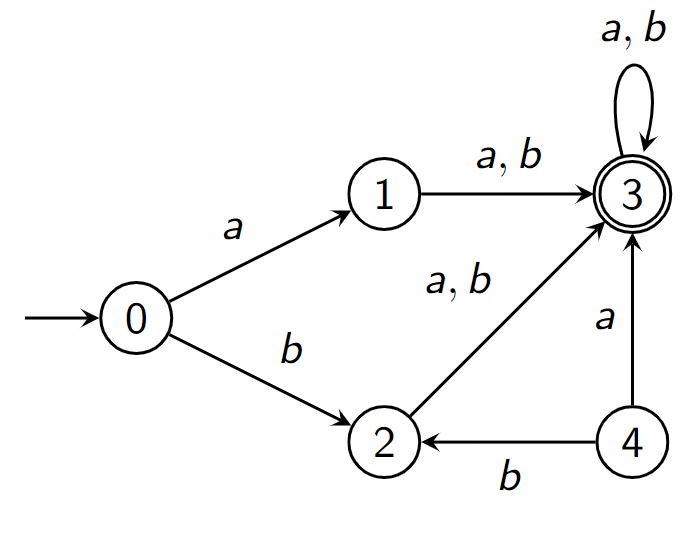
\includegraphics[scale=0.4]{img/cap2/min.png}
    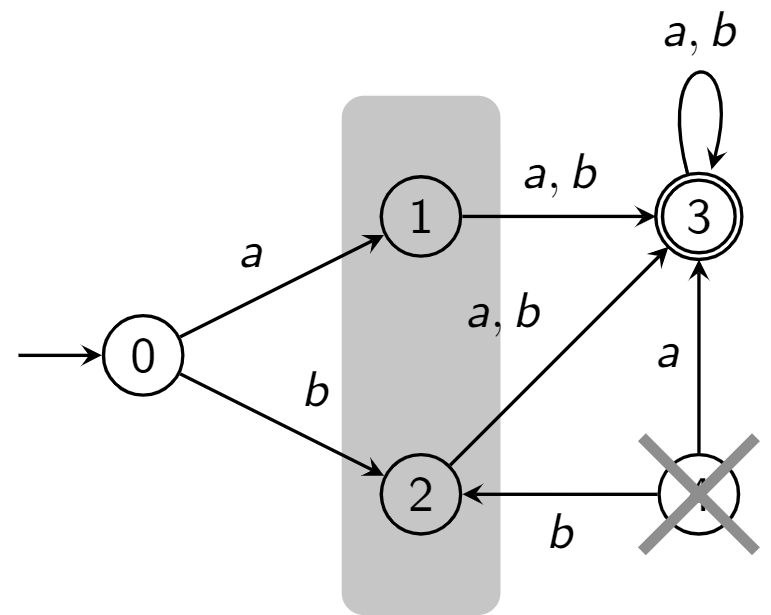
\includegraphics[scale=0.1755]{img/cap2/min_2.png}
    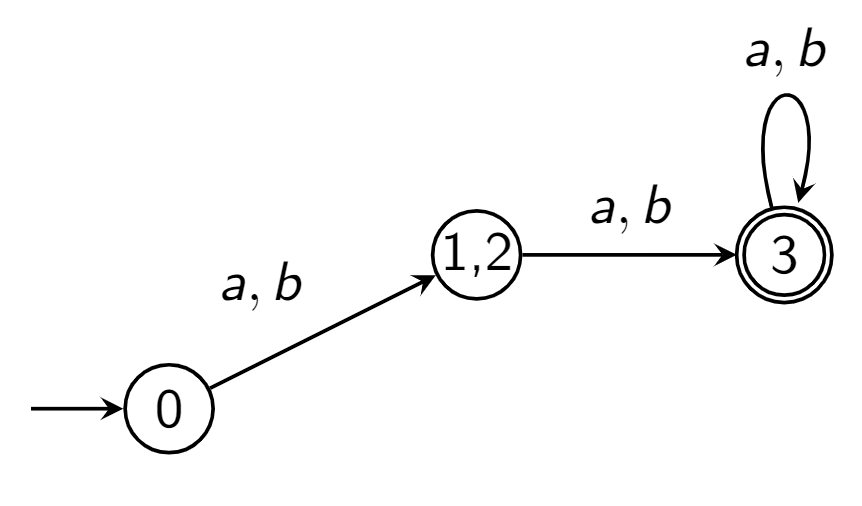
\includegraphics[scale=0.35]{img/cap2/min_3.png}
    \caption{Idea de minimización}
\end{figure}

\begin{enumerate}
    \item Eliminar estados inaccesibles.
          \begin{itemize}
              \item Fácil de realizar y no cambia el lenguaje del autómata finito.
          \end{itemize}
    \item Colapsar estados ``equivalentes''.
          \begin{itemize}
              \item ¿Cómo sabemos cuáles estados colapsar y cúales no?
          \end{itemize}
\end{enumerate}

\ejemplo{}{}{
    Considere el siguiente autómata:
    \img{img/cap2/ejemplo5_1.png}{0.4}
    Podemos:
    \begin{itemize}
        \item Colapsar estados 1 y 2.
        \item Colapsar estados 3 y 4.
    \end{itemize}
    \begin{figure}[H]
        \centering
        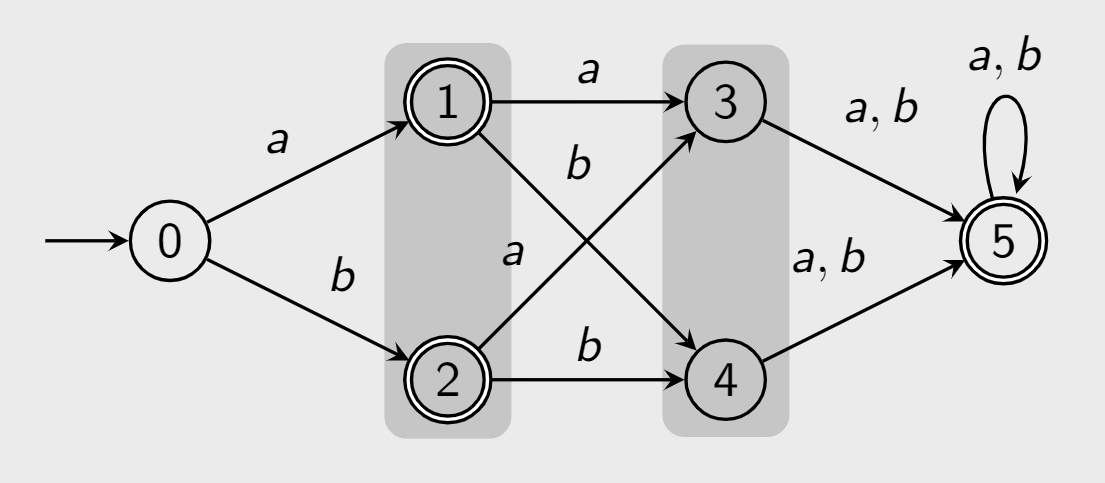
\includegraphics[scale=0.1755]{img/cap2/ejemplo5_2.png}
        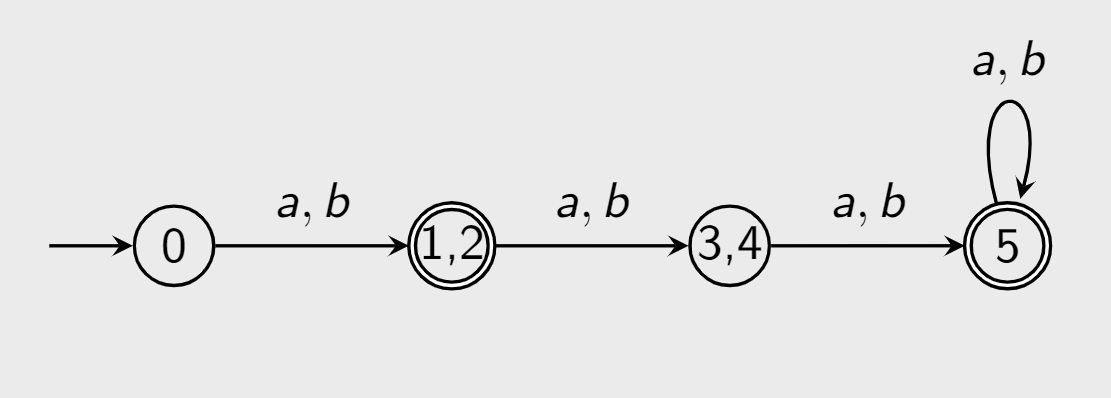
\includegraphics[scale=0.4]{img/cap2/ejemplo5_3.png}
    \end{figure}
}

\ejemplo{}{}{
    Considere el siguiente autómata:
    \img{img/cap2/ejemplo6_1.png}{0.4}
    Podemos:
    \begin{itemize}
        \item Colapsar estados 1 y 2.
        \item Colapsar estados 3, 4 y 5.
    \end{itemize}
    \begin{figure}[H]
        \centering
        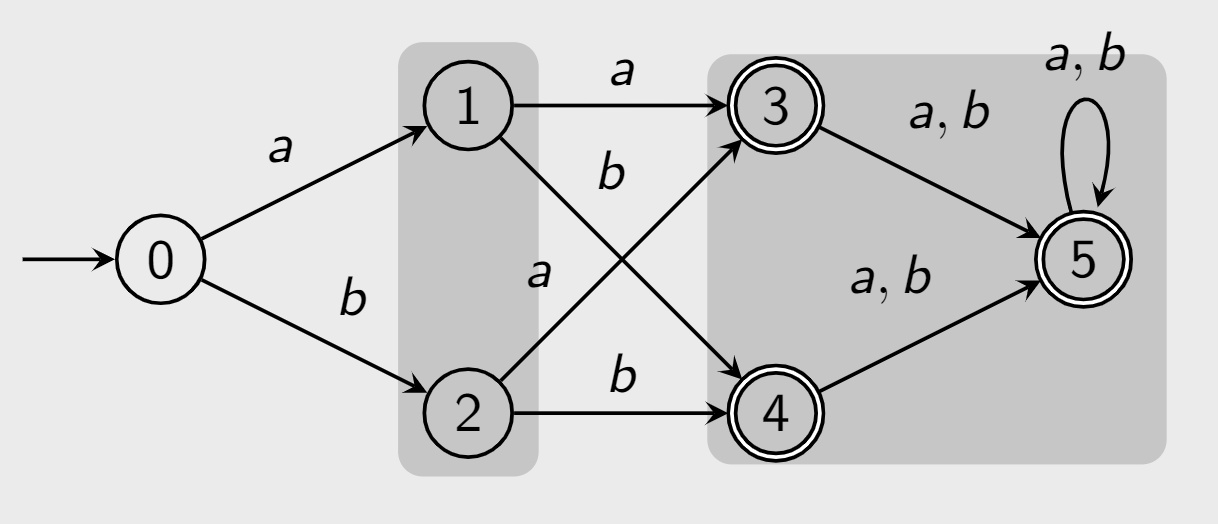
\includegraphics[scale=0.1755]{img/cap2/ejemplo6_2.png}
        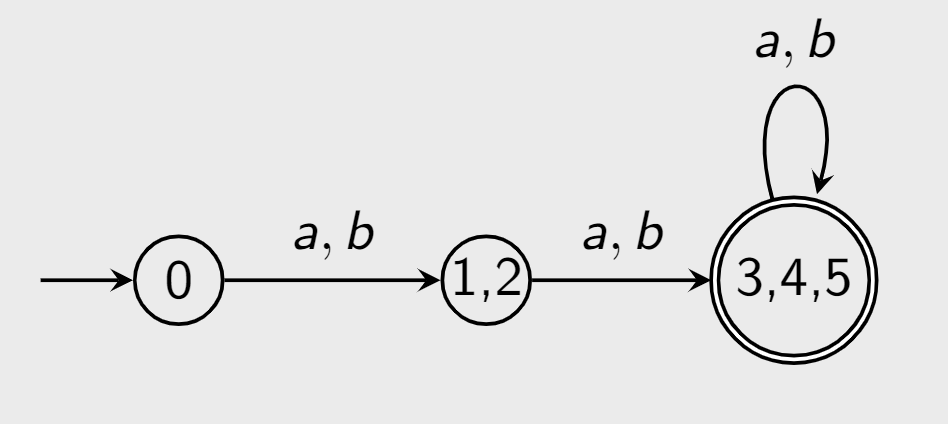
\includegraphics[scale=0.4]{img/cap2/ejemplo6_3.png}
    \end{figure}
}

\subsubsection{Colapsar estados}

\paragraph{Definición.} Sea $\ca{A} = (Q, \Sigma, \delta, q_0, F)$ un DFA.

Se define la \textbf{función de transición extendida} $\hat{\delta}: Q \times \Sigma^* \rightarrow Q$ inductivamente como:
\alignformula{
    \begin{array}{rll}
        \hat{\delta}(q, \epsilon)  & \stackrel{\text { def }}{\equiv} & q                             \\
        \hat{\delta}(q, w \cdot a) & \stackrel{\text { def }}{\equiv} & \delta(\hat{\delta}(q, w), a)
    \end{array}
}

\paragraph{Definición.} Decimos que $p$ y $q$ son \textbf{indistingibles} ($p \approx_\ca{A} q$) si:
\alignformula{
    p \approx_\mathcal{A} q \quad \text { ssi } \quad(\hat{\delta}(p, w) \in F \Leftrightarrow \hat{\delta}(q, w) \in F), \text { para todo } w \in \Sigma^* .
}
Decimos que $p$ y $q$ son \textbf{distingibles} si NO son indistingibles ($p \not\approx_\ca{A} q$).

\paragraph{Recordatorio relaciones de equivalencia.} Una relación $\approx_R$ sobre un conjunto $X$ se dice de \textbf{equivalencia} si es:
\begin{itemize}
    \item \textbf{Refleja:} $\forall p \in X.\ p \approx_R p$
    \item \textbf{Simétrica:}  $\forall p,q \in X.$ si $p \approx_R q$ entonces $q \approx_R p$.
    \item \textbf{Transitiva:} $\forall p,q,r \in X.$ si $p \approx_R q$ y $q \approx_R r$, entonces $p \approx_R r$.
\end{itemize}

Para un elemento $p \in X$ se define su \textbf{clase de equivalencia} según $\approx_R$ como:
$$
    [p]_{\approx_R} = \{q \mid q \approx_R p\}
$$
Una función $f: X \to X$ se dice \textbf{bien definida} sobre $\approx_R$ si:
$$
    p \approx_R q \quad \text{entonces} \quad f(p) \approx_R f(q)
$$

\paragraph{Propiedades de $\approx_\ca{A}$.} Tenemos que:
\begin{itemize}
    \item $\approx_\ca{A}$ es una \textbf{relación de equivalencia}, es decir, es refleja, simétrica y transitiva.
    \item Cada estado $p \in Q$ esta en exactamente una clase de equivalencia:
          $$
              [p]_{\approx_\ca{A}} = \{q \mid q \approx_\ca{A} p\}
          $$
    \item Para todo $a \in \Sigma$ la función $\delta(\cdot, a): Q \to Q$ esta \textbf{bien definida} sobre $\approx_\ca{A}$:
          $$
              p \approx_\ca{A} q \quad \text{entonces} \quad \delta(p,a) \approx_\ca{A} \delta(q,a)
          $$
\end{itemize}

\paragraph{El autómata cuociente.} Para un DFA $\ca{A} = (Q,\Sigma,\delta,q_0,F)$ se define el DFA:
\alignformula{
    \ca{A} / \approx \;= (Q_\approx, \Sigma, \delta_\approx, q_\approx, F_\approx)
}
\begin{itemize}
    \item $Q_{\approx}=\left\{[p]_{\approx_\mathcal{A}} \mid p \in Q\right\}$
    \item $\delta_{\approx}\left([p]_{\approx_\mathcal{A}}, a\right)=[\delta(p, a)]_{\approx_\mathcal{A}}$
    \item $q_{\approx}=\left[q_0\right]_{\approx_\mathcal{A}}$
    \item $F_{\approx}=\left\{[p]_{\approx_\mathcal{A}} \mid p \in F\right\}$
\end{itemize}

\teorema{}{}{
    Para todo autómata finito determinista $\ca{A}$ se cumple que:
    $$
        \ca{L}(\ca{A}) = \ca{L}(\ca{A} / \approx)
    $$
}

\paragraph{Demostración.} Queda como ejercicio propuesto al lector.

\subsubsection{Algoritmo de minimización}

El objetivo es buscar los pares de estados que son \textbf{distingibles}:
\begin{enumerate}
    \item Construya una tabla con los pares $\{p,q\}$ inicialmente sin marcar.
    \item Marque $\{p,q\}$ si $p \in F$ y $q \notin F$ o viceversa.
    \item Repita este paso hasta que no hayan más cambios:
          \begin{itemize}
              \item Si $\{p,q\}$ no están marcados y $\{\delta(p,a),\delta(q,a)\}$ estan marcados para algún $a \in \Sigma$, entonces marque $\{p,q\}$.
          \end{itemize}
    \item Al terminar, $p \not\approx_\ca{A} q$ si, y sólo si, la entrada $\{p,q\}$ está marcada.
\end{enumerate}

Veamos como funciona el algoritmo. Considere el siguiente autómata y una tabla que relacione todos los pares de estados:

\img{img/cap2/amin1.png}{0.175}

\begin{multicols}{2}
    \begin{enumerate}

        \item Construya una tabla con los pares $\{p,q\}$ inicialmente sin marcar.
              \img{img/cap2/amin2.png}{0.175}

        \item Marque $\{p,q\}$ si $p \in F$ y $q \not\in F$ o viceversa.
              \img{img/cap2/amin3.png}{0.175}
    \end{enumerate}
\end{multicols}

\begin{enumerate}
    \item[3.] Repita este paso hasta que no hayan más cambios:
        \begin{itemize}
            \item Si $\{p,q\}$ no están marcados y $\{\delta(p,a), \delta(q,a)\}$ estan marcados para algún $a \in \Sigma$, entonces marque $\{p,q\}$.
        \end{itemize}
        \begin{figure}[H]
            \centering
            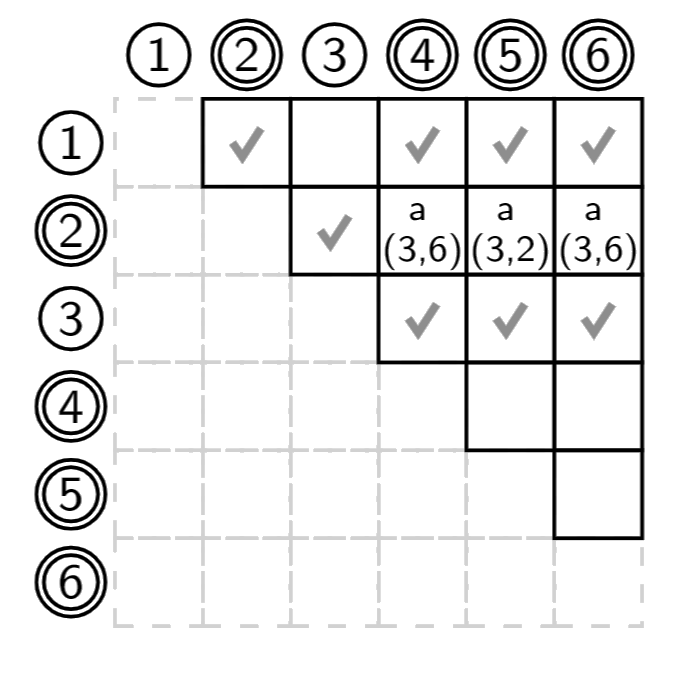
\includegraphics[scale=0.175]{img/cap2/amin4.png}
            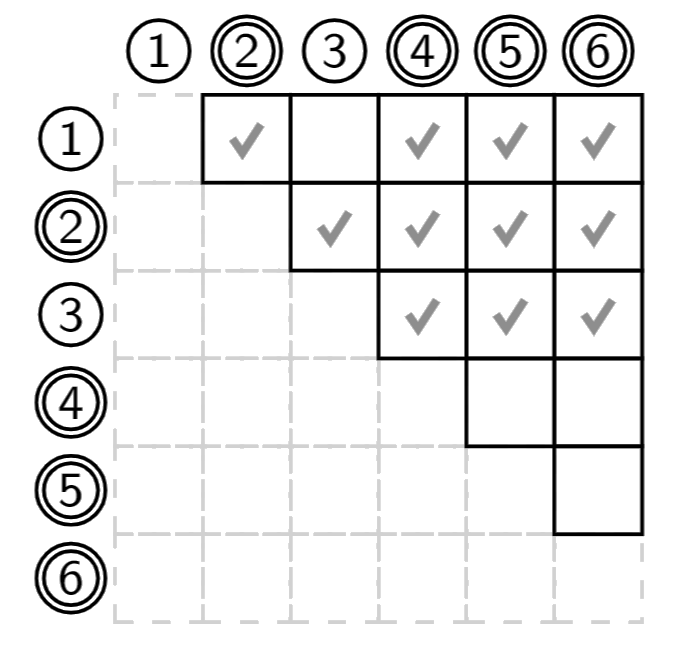
\includegraphics[scale=0.175]{img/cap2/amin5.png}
            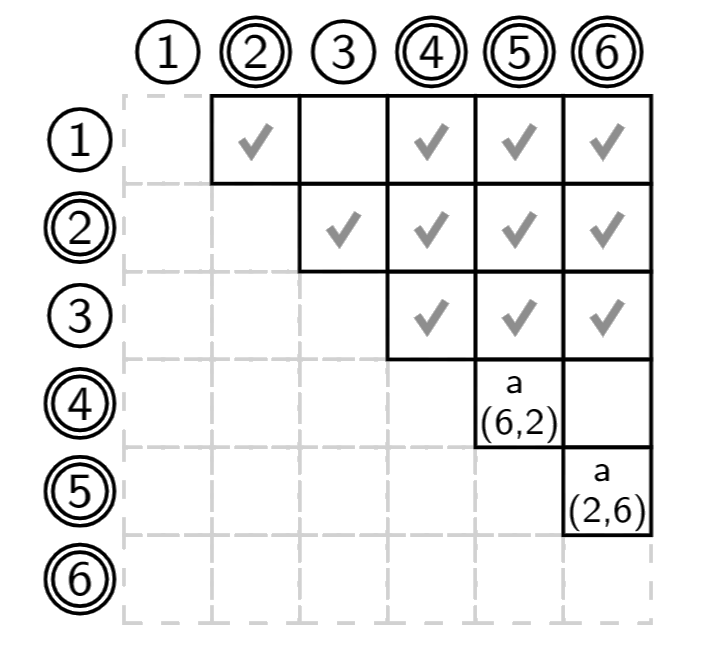
\includegraphics[scale=0.175]{img/cap2/amin6.png}
            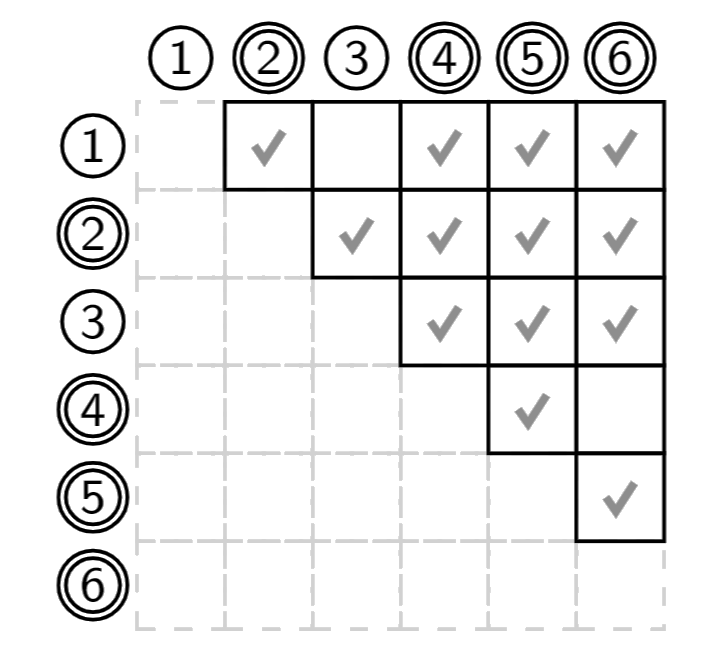
\includegraphics[scale=0.175]{img/cap2/amin7.png}
            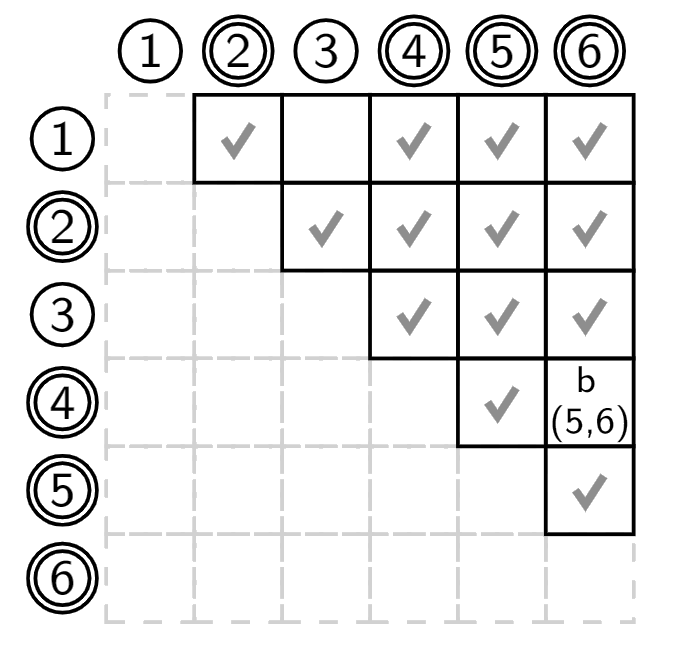
\includegraphics[scale=0.175]{img/cap2/amin8.png}
            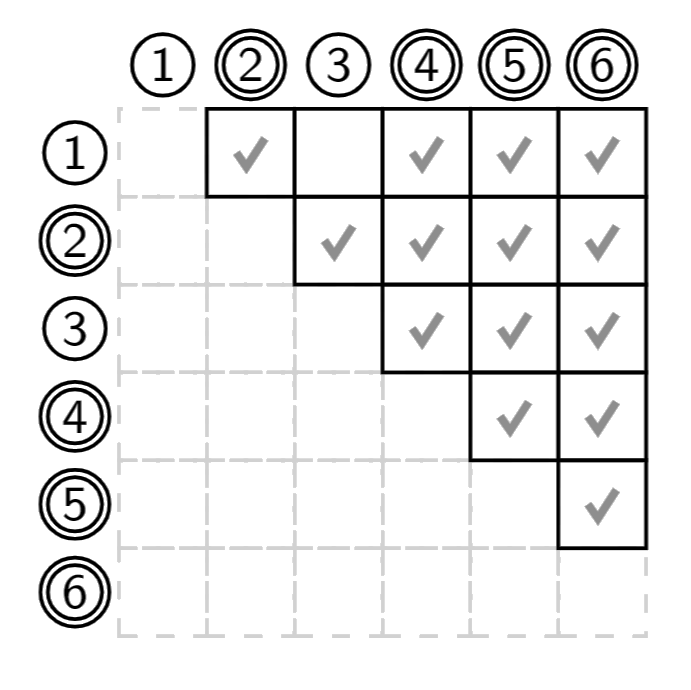
\includegraphics[scale=0.175]{img/cap2/amin9.png}
        \end{figure}
\end{enumerate}

\begin{enumerate}
    \item[4.] Al terminar, $p \not\approx_\ca{A} q$ si, y sólo si, la entrada $\{p,q\}$ está marcada.
\end{enumerate}

Así, vemos que los pares indistingibles son todas las entradas \textbf{NO} marcadas.

\subsection{Teorema de Myhill-Nerode}

La sección anterior deja muchas incógnitas:
\begin{enumerate}
    \item ¿Cómo sabemos si el autómata del algoritmo es un \textbf{mínimo}?
    \item Dado $L$, ¿existe un \textbf{único} autómata mínimo?
    \item Dado un $\ca{A}$, ¿es posible \textbf{construir} un autómata mínimo equivalente?
\end{enumerate}

En esta sección, demostraremos que:
\begin{itemize}
    \item El autómata con el mínimo de estados es \textbf{único}.
    \item El algoritmo de minimización \textbf{siempre} construye el autómata mínimo.
\end{itemize}

\paragraph{Estrategia.} Para demostrar lo dicho anteriormente, seguimos los siguientes pasos:
\begin{enumerate}
    \item Desde un DFA $\ca{A}$, definiremos una relación de equivalencia (RE) $\equiv_\ca{A}$ entre palabras en $\Sigma^*$.
    \item Desde una RE $\equiv$ entre palabras, construiremos un DFA $\ca{A}_\equiv$.
    \item A partir de un lenguaje $L$, definiremos una RE $\equiv_L$.
    \item $\ca{A}_{\equiv_L}$ define el autómata con la \textbf{menor cantidad de estados}.
    \item $\ca{A}_{\equiv_L}$ es equivalente al resultado de nuestro \textbf{algoritmo de minimización}.
\end{enumerate}

\subsubsection{Relaciones de Myhill-Nerode}

Sea $L \subseteq \Sigma^*$ cualquier lenguaje.

\paragraph{Definición.} Una relación de equivalencia $\equiv$ en $\Sigma^*$ es de \textbf{Myhill-Nerode} para $L$ si:
\begin{enumerate}
    \item $\equiv$ es una \textbf{congruencia por la derecha}.
    \item $\equiv$ \textbf{refina} $L$.
    \item El número de clases de equivalencia de $\equiv$ es \textbf{finita}.
\end{enumerate}

A partir de una relación $\equiv$ de Myhill-Nerode podemos construir un DFA $\ca{A}_\equiv$.
\alignformula{
    \ca{A} \quad &\Rightarrow \quad \equiv_\ca{A} \\
    \equiv \quad &\Rightarrow \quad \ca{A}_\equiv
}

\paragraph{Construcción del DFA $\ca{A}_\equiv$.} Dada una relación de Myhill-Nerode $\equiv$ para $L \subseteq \Sigma^*$, definimos el autómata:
\alignformula{
    \ca{A}_\equiv = (Q_\equiv, \Sigma, \delta_\equiv, q_\equiv, F_\equiv)
}
\begin{itemize}
    \item $Q_{\equiv}=\left\{[w]_{\equiv} \mid w \in \Sigma^*\right\}$
    \item $q_{\equiv}=[\epsilon]_{\equiv}$
    \item $F_{\equiv}=\left\{[w]_{\equiv} \mid w \in L\right\}$
    \item $\delta_{\equiv}\left([w]_{\equiv}, a\right)=[w a]_{\equiv}$
\end{itemize}

\teorema{}{}{
    Cada cualquier $L \subseteq \Sigma^*$, tenemos que
    $$
        \ca{L}(\ca{A}_\equiv) = L
    $$
}

Podemos establecer que $\ca{A} \; \Rightarrow \; \equiv_\ca{A}$ y $\equiv \; \Rightarrow \; \ca{A}_\equiv$ son procesos inversos, conclusión que se ilustra en el siguiente teorema.

\teorema{}{}{
    \begin{enumerate}
        \item Si $\ca{A}$ es un DFA que acepta $L$ y si construimos:
              $$
                  \ca{A} \quad \Rightarrow \quad \equiv_\ca{A} \quad \Rightarrow \quad \ca{A}_{\equiv_\ca{A}}
              $$
              entonces $\ca{A}$ es \textbf{isomorfo} (``equivalente'') a $\ca{A}_{\equiv_\ca{A}}$.

        \item Si $\equiv$ es una relación de Myhill-Nerode para $L$ y si construimos:
              $$
                  \equiv \quad \Rightarrow \quad \ca{A}_\equiv \quad \Rightarrow \quad \equiv_{\ca{A}_\equiv}
              $$
              entonces la relación $\equiv$ es \textbf{equivalente} a $\equiv_{\ca{A}_\equiv}$.
    \end{enumerate}
}

La demostración de ambos teoremas queda propuesto como ejercicio al lector.

\subsubsection{Camino al teorema}
Antes de enunciar el Teorema de Myhill-Nerode, debemos aún mencionar algunas definiciones.

\paragraph{Definición.} Dado un lenguaje $L \subseteq \Sigma^*$, se define la relación de equivalencia $\equiv_L$ como:
\alignformula{
    u \equiv_L v \quad \text{ssi} \quad(u \cdot w \in L \Leftrightarrow v \cdot w \in L) \quad \forall w \in \Sigma^*
}

\ejemplo{}{}{
    Sea $L = (ab)^*$. Algunas clases de equivalencia para $L$ son:
    \begin{itemize}
        \item $[\epsilon]_{\equiv_L}=\{\epsilon, a b, a b a b, a b a b a b, \ldots\}$.
        \item $[a]_{\equiv_L}=\{a, a b a, a b a b a, a b a b a b a, \ldots\}$.
        \item $[b]_{\equiv_L}=\{b, b b, b a, a b b, \ldots\}$
    \end{itemize}
}

\paragraph{Propiedades.} $\equiv_L$ se caracteriza por:
\begin{enumerate}
    \item Ser una \textbf{congruencia por la derecha}:
          $$
              u \equiv_L v \text { entonces } u \cdot w \equiv_L v \cdot w \quad \forall w \in \Sigma^*
          $$
    \item Refinar a $L$:
          $$
              u \equiv_L v \text { entonces }(u \in L \Leftrightarrow v \in L)
          $$
    \item Si $\equiv$ es una congruencia por la derecha y refina $L$, entonces $\equiv$ \textbf{refina} a $\equiv_L$:
          $$
              u \equiv v \text { entonces } u \equiv_L v
          $$
\end{enumerate}

Con todo lo anterior, estamos en condiciones de enunciar el teorema.

\teorema{}{}{
    Sea $L \subseteq \Sigma^*$. Las siguientes propiedades son equivalentes:
    \begin{enumerate}
        \item $L$ es \textbf{regular}.
        \item Existe una \textbf{relación de Myhill-Nerode} para $L$.
        \item La relación $\equiv_L$ tiene una cantidad \textbf{finita} de clases de equivalencia.
    \end{enumerate}
}

\paragraph{Demostración teorema 10.} Del punto 1 al 2, tenemos que si $L$ es regular, entonces:
\begin{itemize}
    \item existe un autómata finito $\ca{A}$ tal que $L = \ca{L}(\ca{A})$.
    \item $\equiv_\ca{A}$ es una relación de Myhill-Nerode para $L$.
\end{itemize}

Del punto 2 al 3, sea $\equiv$ una relación de Myhill-Nerode para $L$, entonces:
\begin{itemize}
    \item $\equiv$ tiene una cantidad finita de clases de equivalencia.
    \item $\equiv_L$ tiene una cantidad finita de clases de equivalencia.
\end{itemize}

Del punto 3 al 1, si $\equiv_L$ tiene una cantidad \textbf{finita} de clases de equivalencia, entonces:
\begin{itemize}
    \item $\equiv_L$ es una relación de Myhill-Nerode para L.
    \item $\ca{A}_{\equiv_L}$ es un autómata finito para $L$. \hfill $\blacksquare$
\end{itemize}

\paragraph{Conclusiones del teorema.} Tenemos que:
\begin{enumerate}
    \item $\equiv_L \; \Rightarrow \; \ca{A}_{\equiv_L}$ produce el autómata con la menor cantidad de estados.
    \item Todo autómata $\ca{A}$ tal que $\equiv_\ca{A} = \equiv_L$ son \textbf{isomorfos} (``equivalentes'').
    \item El \textbf{algoritmo de minimización} produce un autómata isomorfo $\ca{A}_{\equiv_L}$.
\end{enumerate}

\paragraph{Demostración punto 3.} Sea $\ca{A} = (Q,\Sigma,\delta,q_0,F)$ un autómata que acepta $L$ ya \textbf{minimizado}:
$$
    \begin{aligned}
        u \equiv_L v \quad & \Leftrightarrow \quad(u \cdot w \in L \Leftrightarrow v \cdot w \in L) \quad \forall w \in \Sigma^*                                                                                                                \\
                           & \Leftrightarrow \quad\left(\hat{\delta}\left(q_0, u \cdot w\right) \in F \Leftrightarrow \hat{\delta}\left(q_0, v \cdot w\right) \in F\right) \quad \forall w \in \Sigma^*                                         \\
                           & \Leftrightarrow \quad\left(\hat{\delta}\left(\hat{\delta}\left(q_0, u\right), w\right) \in F \Leftrightarrow \hat{\delta}\left(\hat{\delta}\left(q_0, v\right), w\right) \in F\right) \quad \forall w \in \Sigma^* \\
                           & \Leftrightarrow \quad \hat{\delta}\left(q_0, u\right) \approx_\mathcal{A} \hat{\delta}\left(q_0, v\right)                                                                                                          \\
                           & \Leftrightarrow \quad \hat{\delta}\left(q_0, u\right)=\hat{\delta}\left(q_0, v\right)                                                                                                                              \\
                           & \Leftrightarrow \quad u \equiv_\mathcal{A} v
    \end{aligned}
$$
\hfill $\blacksquare$

\subsection{Autómatas en dos direcciones}

\subsubsection{Definición de un 2DFA}

\fig{img/cap2/2dfa.png}{0.2}{Representación de un 2DFA}

\paragraph{Definición.} Un autómata finito determinista en 2 direcciones (2DFA) es una estructura:
\alignformula{
    \mathcal{A}=\left(Q, \Sigma, \vdash, \dashv, \delta, q_0, q_f\right)
}
\begin{itemize}
    \item $Q$ es un conjunto finito de estados.
    \item $\Sigma$ es el alfabeto del input.
    \item $\vdash$ y $\dashv$ son las marcas (símbolos) iniciales y finales.
    \item $\delta: Q \times(\Sigma \cup\{\vdash, \dashv\}) \rightarrow Q \times\{\leftarrow, \rightarrow\}$ es la \textbf{función parcial de transición}.
    \item $q_0$ es el estado inicial.
    \item $q_f$ es el estado final.
\end{itemize}

\ejemplo{}{}{
    \img{img/cap2/ejemplo7.png}{0.225}
}

\paragraph{Configuración.} Sea $\ca{A}$ un 2DFA y $w = a_1 \ldots a_n \in \Sigma^*$ un input. Definimos $a_0 =\ \vdash$ y $a_{n+1} =\ \dashv$ tal que el input se define como:
\alignformula{
    a_0 a_1 \ldots a_n a_{n+1} =\ \vdash \cdot\ w\ \cdot\ \dashv
}
Una \textbf{configuración} de $\ca{A}$ sobre $w$ viene dado por un par:
\alignformula{
    (q, i) \in Q \times\{0, \ldots, n+1\}
}
\begin{itemize}
    \item $q$ es el \textbf{estado actual} del autómata.
    \item $i$ es la \textbf{posición actual} de la cabeza lectora.
\end{itemize}

Se define la relación de \textbf{siguiente configuración} $\stackrel{\mathcal{A}}{\longmapsto}$ de $\ca{A}$ sobre $w$ como:
\alignformula{
    (p, i) \stackrel{\mathcal{A}}{\longmapsto}(q, j)
}
tal que:
\begin{itemize}
    \item Si $\delta(p, a_i) = (q, \rightarrow)$, entonces $(p, i) \stackrel{\mathcal{A}}{\longmapsto}(q, i+1)$.
    \item Si $\delta\left(p, a_i\right)=(q, \leftarrow)$, entonces $(p, i) \stackrel{\mathcal{A}}{\longmapsto}(q, i-1)$.
\end{itemize}

\paragraph{Ejecución.} Una ejecución (o \textit{run}) $\rho$ de $\ca{A}$ sobre $w$ es una secuencia de configuraciones:
\alignformula{
    \rho:\left(p_0, i_0\right) \rightarrow\left(p_1, i_1\right) \rightarrow \ldots \rightarrow\left(p_m, i_m\right)
}
donde $p_0 = q_0$ y $i_0 = 0$. Además, $\left(p_j, i_j\right) \stackrel{\mathcal{A}}{\longmapsto}\left(p_{j+1}, i_{j+1}\right) \quad \forall j \in[0, m-1]$. \medbreak

Una ejecución $\rho$ de $\ca{A}$ sobre $w$ es de \textbf{aceptación} si:
\alignformula{
    p_m=q_f \quad y \quad i_m=n+1
}

\paragraph{Aceptación.} Decimos que $\ca{A}$ \textbf{acepta} $w$ si hay una ejecución de $\ca{A}$ sobre $w$ que es de \textbf{aceptación}. Así, el \textbf{lenguaje aceptado} por $\ca{A}$ se define como:
\alignformula{
    \mathcal{L}(\mathcal{A})=\left\{w \in \Sigma^* \mid \mathcal{A} \text { acepta } w\right\}
}

\textbf{Ojo:} Notemos que un 2DFA puede pasar por error o NO parar nunca.

\subsubsection{2DFA vs DFA}

Para todo lenguaje regular $L$ existe un 2DFA $\ca{A}$:
\alignformula{
    L = \ca{L}(\ca{A})
}
En otras palabras, DFA $\subseteq$ 2DFA. \bigbreak

¿Son los 2DFA más poderosos que los DFA? En esta sección, demostraremos que no, es decir, pueden representar al mismo conjunto de lenguajes.

\paragraph{¿Cuánta información puede almacenar un 2DFA?} Veamos la siguiente figura:
\begin{multicols}{2}
    \img{img/cap2/2dfa_1.png}{0.2}

    \textit{``Cada vez que $\ca{A}$ cruce de $w$ a $u$ en el estado $p$, $\ca{A}$ cruzará de regreso en el estado $q$''}. \medbreak

    Este comportamiento solo depende de $u$, y no de $w$:
    \img{img/cap2/2dfa_2.png}{0.175}
\end{multicols}

Para cada $u \in \Sigma^*$, definimos la función $T_u: Q \cup\{\bullet\} \rightarrow Q \cup\{\perp\}$ tal que:
\begin{itemize}
    \item $T_u(p) = q \quad$ si, y sólo si, $\quad$ desde $(p, |u|)$ cruza en la configuración $(q, |u|+1)$.
    \item $T_u(p) = \perp \quad$ si, y sólo si, $\quad$ desde $(p, |u|)$ nunca cruza de $u$.
    \item $T_u(\bullet) = q \quad$ si, y sólo si, $\quad$ desde $(q_0,0)$ cruza por primera vez con $(q, |u| + 1)$.
    \item $T_u(\bullet) = q \quad$ si, y sólo si, $\quad$ desde $(q_0,0)$ cruza por primera vez con $(q, |u| + 1)$.
    \item $T_u(\bullet) = \perp \quad$ si, y sólo si, $\quad$ desde $(q_0,0)$ nunca cruza de $u$.
\end{itemize}

\begin{multicols}{2}
Suponga que ahora tenemos una palabra $v$ tal que:
$$
    T_v = T_u
$$
\img{img/cap2/2dfa_3.png}{0.2}

Entonces, $v$ es \textbf{indistingible} de $u$ según $\ca{A}$. En otras palabras:
$$
    u \cdot w \in \mathcal{L}(\mathcal{A}) \Leftrightarrow v \cdot w \in \mathcal{L}(\mathcal{A}) \quad \text { para todo } w \in \Sigma^*
$$
Lo anterior tiene conexión con las relaciones de Myhill-Nerode, que vimos en una sección anterior.
\end{multicols}
Luego, respecto a la función $T_u$ podemos decir que:
\begin{enumerate}
    \item Definimos la relación $\equiv_T$ entre palabras en $\Sigma^*$ tal que:
    $$
    u \equiv_T v \text { si, y solo si, } \quad T_u=T_v
    $$
    es una \textbf{relación de equivalencia}.
    \item $\equiv_T$ es una \textbf{congruencia por la derecha}:
    $$
    u \equiv_T v \Rightarrow \forall w \cdot u \cdot w \equiv_T v \cdot w
    $$
    \item $\equiv_T$ \textbf{refina} a $\ca{L}(\ca{A})$:
    $$
    u \equiv T v \Rightarrow(u \in L \Leftrightarrow v \in L)
    $$
    \item La relación $\equiv_T$ tiene una \textbf{cantidad finita} de clases de equivalencia:
    $$
    T: Q \cup\{\bullet\} \rightarrow Q \cup\{\perp\}
    $$
    Así, $\equiv_{\ca{L}(\ca{A})}$ también tiene una cantidad \textbf{finita} de \textbf{clases de equivalencia}.
\end{enumerate}

\teorema{}{}{
    Para todo 2DFA $\ca{A}$ existe un DFA $\ca{A}'$ tal que:
    $$
    \ca{L}(\ca{A}) = \ca{L}(\ca{A}')
    $$
    En otras palabras, 2DFA $\equiv$ DFA.
}

El DFA del teorema anterior se construye usando el Teorema de Myhill-Nerode a partir de las funciones $T_u$. \medbreak

La demostración del teorema y la construcción queda como ejercicio propuesto para el lector.